The complexity of a \ac{LBA} increases with the complexity of the system it has
to work with.
Consider a load balancing algorithm that computes the target worker for a task,
where the size of the tasks are equal, the workers have the same capabilities
and the number of overall tasks is known.
Such an algorithm is not of complexity.
In fact, it can be implemented by a simple mathematical equation:
\begin{equation}
    i = j \% |W|
\end{equation}
Where $i$ is the number of the worker instance in set $W$ that will be assigned
with the task number $j$.
Though, such an environment is unlikely.

In todays systems, the size of a task can often not be predicted.
Algorithms like ``min-min'' and ``max-min''
\cite{anInDepthAnal} are not applicable to most systems, because
with these algorithms, the complete set of tasks must be known before scheduling
them.
In most environments, this is not possible.

The capabilities of a worker instance may be known, but as tasks come in and are
assigned to workers, an algorithm has to implement some book-keeping to know
which worker has the least load at a given point in time.
This is of moderate complexity, though having only one load balancer in a large
ecosystem is highly unlikely, as it would be a single point of failure.
Instead, multiple load balancers are used.
Because of this, some synchronization method between the book-keeping of each
load balancer must be introduced to ensure the integrity of the load data on
each load balancer node.

If worker instance $W_1$ has the least load at time $t_1$, the load balancer
$L_1$ might assign a number of tasks to it in $t_2$.
After that, $L_1$ must notify $L_2$ about the new load on $W_1$, which it does
in $t_3$.
In the meantime, load balancer $L_2$ might need to assign another set of tasks,
which it assignes to $W_1$ in $t_2$, because it does not know yet that $W_1$
isn't the least loaded worker anymore.
This causes $W_1$ to become overloaded in $t_3$.

% TODO: Graphic on timing example from above

\subsection{Random load balancing}

A cheap load balancing strategy is randomizing the target.
\begin{equation}
    i = rand() \% |W|
\end{equation}
Which has several advantages over other approaches:
\begin{itemize}
    \item Simplicity
    \item Few edge cases
    \item Easy failover
    \item Works distributed
\end{itemize} % TODO: cite http://www.codemesh.io/codemesh/tyler-mcmullen ?
These properties are rather easy to replicate with non-random load balancing
algorithms, except the last one.

In a common load balancing environment, having only one load balancer
distributing tasks between worker instances is naive.
Commonly, at least one fail-over is deployed, sometimes several.
Also, in a large system, load balancers might be spread not only over server
racks but rather continents.
Making load balancers work with each other and synchronize state information
introduces high complexity.

Anyways, distributing load randomly does not guarantee the best distributing
over a given set of notes, neither with one load balancer nor with many.
It is even possible that a small set of workers are assigned
with a huge number of tasks while other workers only handle a very small number
of tasks, resulting in a high load on some machines while others idle.

The desireable state is that each machine has the same workload, resulting in a
perfect distribution of load over all machines.
With an algorithm randomly assigning work to workers, the possibility exists
that the system ends up in an unbalanced state.
Though this is very unlikely, we can do better.

\subsection{\ac{RR}}

Another cheap load balancing strategy might be \ac{RR}.
\begin{equation}
    i = number\_of(T) \% |W|
\end{equation}
As \ac{RR} is a static algorithm \cite{availabilityLBinCC},
it yields, as with randomized load balancing, problems in distributed
environments, where not one but many load balancers are applied to a network of
servers.

Also, as uniform tasks only occur in a perfect world, \ac{RR} load balancing
might result in overloaded servers as well.

\subsection{\ac{JSQ}}

A known load balancing algorithm is \ac{JSQ}.

With this algorithm, the load balancing mechanism implements some book-keeping
mechanism how many jobs are in the queues of the worker instances and selects
the instance with the shortest queue for a new task.

If this algorithm is applied in a non-distributed environment, it behaves
exactly like \ac{RR} \ref{chap:algo:rr}.
Applying it with several load-balancers, though, might yield some better
results, though synchronization must be implemented carefully.
As synchronization is rather expensive, one might implement a scheduled
synchronization which causes the instances to synchronize state information in a
periodic manner.
However, this can result in a ``herd effect'' in distributed environments,
where a subset of machines is either underutilized or overloaded with tasks.
This is caused by the old information of how the nodes are
utilized as described in.
Mechanisms exists to use this old information to estimate the current situation
and improve the decisions of the load balancing (\cite{inpSLoadInfo}).
The LI framework as introduced in \cite{inpSLoadInfo} improves load distribution
if the information about the utilization of the nodes is old and therefor
prevents the ``herd effect'' mentioned earlier.

As synchronization might be to complex and faulty to implement, querying the
servers for their queue length might be an alternative.
With a querying-mechanism, synchronization, and therefor blocking, would be
omitted.
However, querying a server instance for its queue length introduces complexity
to the servers and might also be a non-trivial task.

Either way, \ac{JSQ} is a valuable option for load balancing in environments
where the request is short-living, like in \ac{DNS}-environments or web servers.

\subsection{\ac{RSJSQ}}

A surprisingly good optimization is the combination of the random load balancing
implementation with \ac{JSQ}.
\begin{equation}
    \begin{aligned}
        x &= rand() \% |I| \\
        y &= rand() \% |I| \\
        i &= \begin{cases}
            x & \text{if } load(W_x) =< load(W_y)\\
            y & \text{if } load(W_x) > load(W_y)\\
        \end{cases}
    \end{aligned}
    \label{eq:randjsq}
\end{equation}
Due to the fact that querying each server for its queue length
might be a non-trivial and expensive task,
selecting two servers randomly (or by a hash function applied to the task, as
stated in \cite{powerOfTwoRandomChoices}) and applying the \ac{JSQ} algorithm on
this subset of servers yields, obviousely, better performance as the number of
queries for the queue length is minimized.

As stated in \cite{powerOfTwoRandomChoices}, \ac{RSJSQ} might result in
$\Theta(log(log(n)))$ tasks on each server, rather than
$\Theta(log(n) / log(log(n)))$, where $n$ is the number of servers in the
environment.

\subsection{Comparing RR, \ac{JSQ} and \ac{RSJSQ}}

For the following comparison of the algorthms \ac{RR}, \ac{JSQ} and \ac{RSJSQ},
they were implemented in the Rust programming languages.
Sample data in form of a CSV file was generated with the code from
Fig. \ref{lst:ruby}

The sample data holds two values in each column: A task name and a time factor.
The former is for simple debugging purposes, the latter is an artificial random
time factor.
It is a number between $1$ and $100$ and specifies how many \emph{ticks} the
task takes to be computed.
The algorithms put one task into the workers on each tick.

\begin{figure}[b!]
    \begin{lstlisting}
    (0...50_000).each do |n|
      r = Random::rand(100) + 1
      puts "Task #{n},#{r}"
    end
    \end{lstlisting}
    \caption{Ruby script to generate random task data}
    \label{lst:ruby}
\end{figure}

\pgfplotsset{every axis legend/.append style={at={(0,0)},anchor=north east}}
\begin{figure}
        \centering
        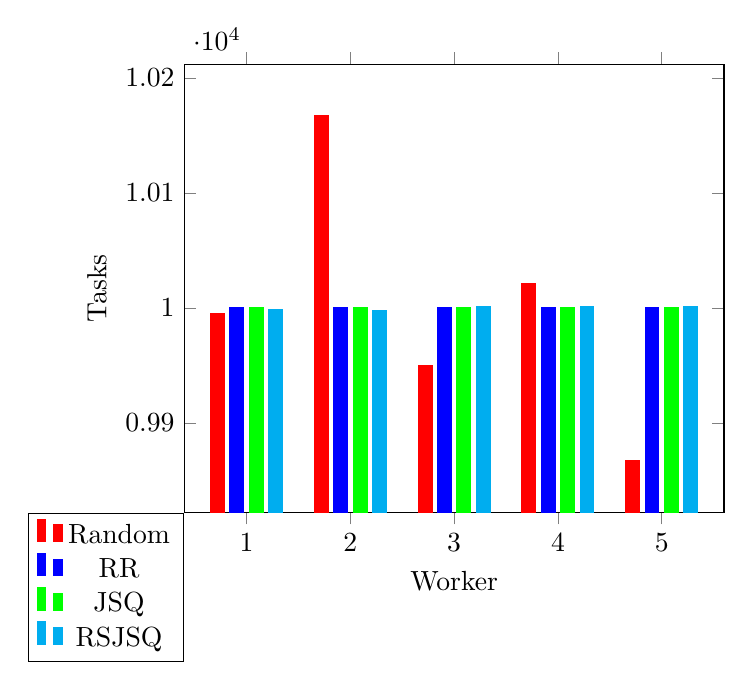
\begin{tikzpicture}
                \begin{axis}[
                        ybar,
                        enlargelimits=0.15,
                        symbolic x coords={0,1,2,3,4,5,6},
                        xtick=data,
                        xlabel={Worker},
                        ylabel={Tasks},
                        nodes near coords align={vertical},
                        bar width=5pt,
                        ]
                        \addplot+[color=red] % Random
                        coordinates {(1,9995) (2,10167) (3,9950) (4,10021) (5,9867)};

                        \addplot+[color=blue] % Roundrobin
                        coordinates {(1,10000) (2,10000) (3,10000) (4,10000) (5,10000)};

                        \addplot+[color=green] % JSQ
                        coordinates {(1,10000) (2,10000) (3,10000) (4,10000) (5,10000)};

                        \addplot+[color=cyan] % select-random-JSQ
                        coordinates {(1,9999) (2,9998) (3,10001) (4,10001) (5,10001)};

                        \legend{Random,RR,JSQ,RSJSQ}
                \end{axis}
        \end{tikzpicture}
        \caption{Task distribution}
        \label{fig:algo:use}
\end{figure}

\begin{figure}[b!]
        \centering
        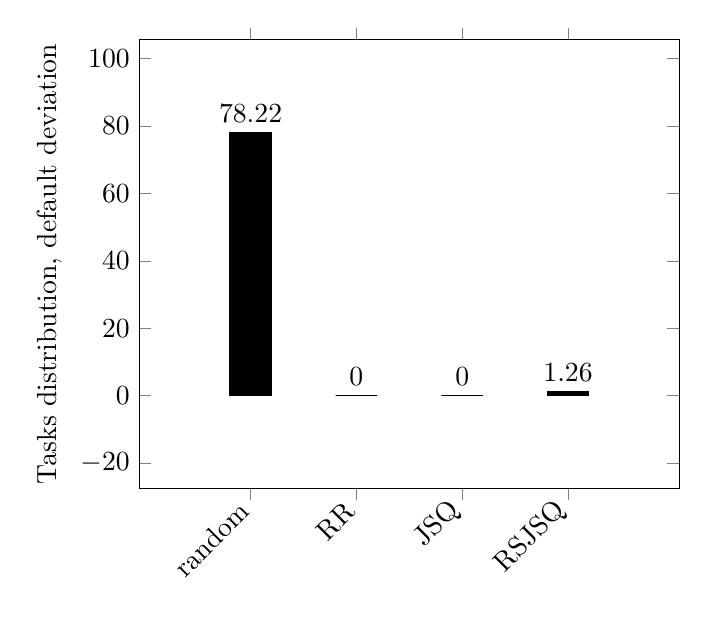
\begin{tikzpicture}
                \begin{axis}[
                        ybar,
                        enlargelimits=0.35,
                        symbolic x coords={random,RR,JSQ,RSJSQ},
                        xtick=data,
                        ylabel={Tasks distribution, default deviation},
                        nodes near coords,
                        nodes near coords align={vertical},
                        x tick label style={rotate=45,anchor=east},
                        bar width=15pt,
                        ]

                        \addplot+[color=black] coordinates
                        {(random,78.22) (RR,0) (JSQ,0) (RSJSQ,1.26)};

                \end{axis}
        \end{tikzpicture}
        \caption{Task distribution, default deviation}
        \label{fig:algo:use:defdev}
\end{figure}

In an environment with one load balancer where tasks can be distributed before
the processing begins, \ac{JSQ} and \ac{RSJSQ} behave exactly like \ac{RR} as
shown in Fig. \ref{fig:algo:use} and Fig. \ref{fig:algo:use:defdev}.
This is not a surprise for \ac{JSQ} (with manual book keeping), as the node with
the least tasks after assigning a task to node $n$ is always the next node:
$(n + 1) \% |N|$.
Surprisingly, \ac{RSJSQ} behaves \emph{almost} like \ac{RR} and \ac{JSQ},
despite the random selection of workers.

If we take the processing of the tasks on the workers into account, though, we
clearly see the improvement of \ac{JSQ} over \ac{RR}.
Each tick one of the tasks inside a worker gets computed, which means that
the time factor gets decremented by $1$.
If a task hits time factor $0$, it gets removed from the tasks queue in the
worker and the next task will be computed on the next tick.
After $50.000$ tasks are pushed into the workers, the current state is printed
out by the implementation (Fig. \ref{fig:algo:time} and
Fig. \ref{fig:algo:time:defdev}).

\begin{figure}
        \centering
        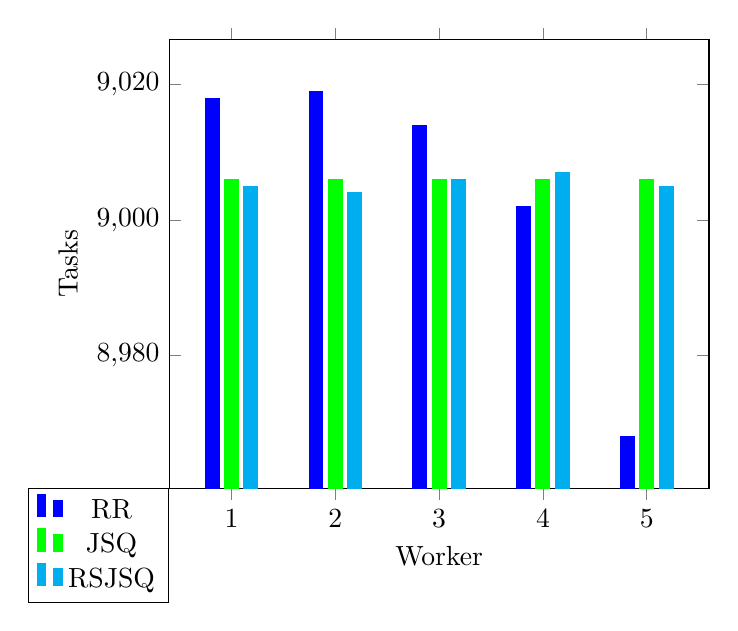
\begin{tikzpicture}
                \begin{axis}[
                        ybar,
                        enlargelimits=0.15,
                        symbolic x coords={0,1,2,3,4,5,6},
                        xtick=data,
                        xlabel={Worker},
                        ylabel={Tasks},
                        nodes near coords align={vertical},
                        bar width=5pt,
                        ]
                        \addplot+[color=blue] % Roundrobin
                        coordinates {(1,9018) (2,9019) (3,9014) (4,9002) (5,8968)};

                        \addplot+[color=green] % JSQ
                        coordinates {(1,9006) (2,9006) (3,9006) (4,9006) (5,9006)};

                        \addplot+[color=cyan] % RSJSQ
                        coordinates {(1,9005) (2,9004) (3,9006) (4,9007) (5,9005)};

                        \legend{RR,JSQ,RSJSQ}
                \end{axis}
        \end{tikzpicture}
        \caption{Task distribution}
        \label{fig:algo:time}
\end{figure}

\begin{figure}[b!]
        \centering
        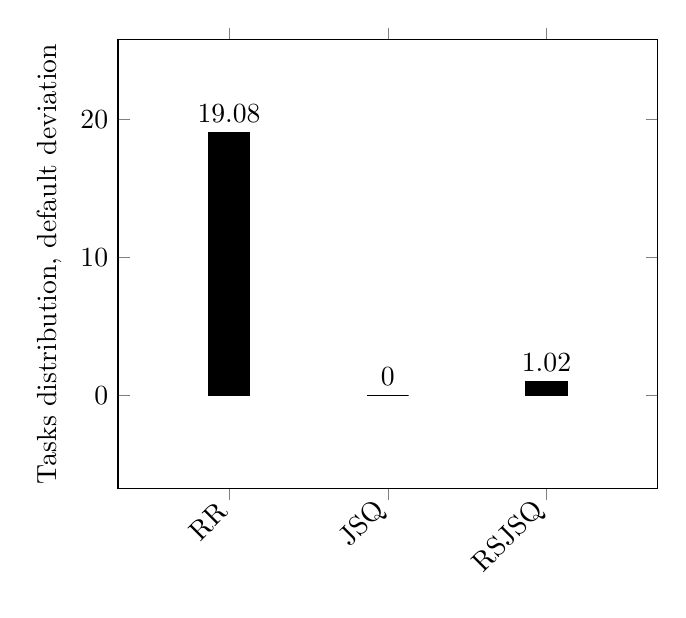
\begin{tikzpicture}
                \begin{axis}[
                        ybar,
                        enlargelimits=0.35,
                        symbolic x coords={random,RR,JSQ,RSJSQ},
                        xtick=data,
                        ylabel={Tasks distribution, default deviation},
                        nodes near coords,
                        nodes near coords align={vertical},
                        x tick label style={rotate=45,anchor=east},
                        bar width=15pt,
                        ]

                        \addplot+[color=black] coordinates
                        {(RR,19.08) (JSQ,0) (RSJSQ,1.02)};

                \end{axis}
        \end{tikzpicture}
        \caption{Task distribution, default deviation}
        \label{fig:algo:time:defdev}
\end{figure}

\subsection{Hash based load balancing}

Another way of distributing load is using a hash algorithm to determine the
target server.
With this approach, each request gets hashed with a hash function.
The result of the hash function can be seen as number.
Taking this number modulo the number of servers yields the index of the target
server.
In his scenario, the number of servers has to be constant.
If a new server is added to the cluster, the modulo operation yields other
servers for the same requests as before, yielding cache effects useless
\cite{medVimeoEngin}.
Another implication of hash based load balancing is that consistent hashing is
less than ideal for load balancing, as requests are not distributed evenly over
content.
Consider a cluster for videos, where each server has a subset of the complete
data.
Naturally, cat videos are more likely to be requested by the user than other
videos, resulting in higher load on the servers holding this particular data.

In \cite{medVimeoEngin} is stated, that as \ac{RSJSQ} was not suiteable for
their problem.
Though, \ac{CHBL} as proposed by \cite{ConsistentHashingWithBoundedLoads} was.

\ac{CHBL} provides some guarantees which are fortunate for dynamic hash based
load balancing in distributed environments.
That is, mostly, an upper bound for the load of each server
\cite{ConsistentHashingWithBoundedLoads}
and some more cache-friendly properties \cite{medVimeoEngin}.
with \ac{CHBL}, distribution of requests is the same as with consistent hashing.

The \ac{CHBL} algorithm was implemented and submitted to the HAProxy HTTP load
balancer open source project and on November 25, HAProxy 1.7.0 was published
with \ac{CHBL} available.
Real world measurements reveal a great benefit from applying \ac{CHBL}, as shown
in \cite{medVimeoEngin}.

% TODO: Work stealing
% TODO: Drafting Algorithm
% TODO: Delayed Binding

% vim: set ts=4 sw=4 tw=0 noet :
